\tightsection{Quality Improvement via Prediction}
\label{improvement}
%Now we can fill in the details of section 3 a bit more.  Figure~\ref{fig:go-overview} shows how prediction and decision-making work in GO.
Having shown that with the attributes we collect, our prediction algorithms can provide close-to-optimal prediction accuracy, we now evaluate the quality improvement resulting from the prediction algorithms. GO's ``transition'' from prediction accuracy to quality improvement is straightforward -- the decision making algorithm simply selects the decision that has the best predicted quality in a predetermined metric. Note that GO always leave a small fraction of traffic to be randomized traffic which is randomly allocated so as to guarantee that each decision will have at least certain fraction of traffic even when it is current not the best decision for any session.

This section quantifies the impact of prediction algorithms on quality improvement. Specifically, we would like to answer two questions:
\begin{packedenumerate}
	\item How much quality improvement does GO make under various scenarios?
	\item How does prediction accuracy impact quality improvement under realistic scenarios?
\end{packedenumerate}

The difference between two questions is that the first question quantifies the impact of parameters of scenarios (e.g., performance heterogeneity) on quality improvement with a fixed prediction algorithm, i.e., GO. The second question quantifies the impact of the goodness of prediction algorithm (i.e., prediction accuracy) on quality improvement, in realistic scenarios. This section begins with a description of our methodology to answer the two questions. Then, we present our results and observations regarding each question.

\tightsubsection{Methodology}
Ideally, to answer these two questions, we need a dataset in which for any session, the quality outcome on each decision is available so that decisions different from the ones that were actually used can be evaluated. However, it is impossible to collect the quality of the same session on multiple decisions simultaneously. In addition, real trace only contains scenarios that happened before, and it is often insufficient to evaluate over a wide range of scenarios.
Alternatively, we use three types of input. Here we briefly describe their intuition and difference. Table~\ref{tab:input} summarizes the features of different types of input. We will present the parameters and setup in detail when using them to answer concrete questions.

\begin{table}[h]
    \begin{tabular}{ccccc}
	\hline
    ~                       & Realistic & Unbiased & Oracle & Randomized \\ \hline
    Type I    & \xmark & \xmark & \cmark & \cmark \\ \hline
    Type II          & \cmark & \cmark & \xmark & \xmark \\ \hline
	Type III & \cmark & \xmark & \cmark & \cmark \\ \hline
    \end{tabular}
	\caption{A summary of features of different types of input.}
\label{tab:input}
\end{table}

\begin{packeditemize}
	\item {\it Type I input: Controlled synthetic input} We need fully controlleable input in which the true outcomes (i.e., ``ground truth'') of multiple decisions are under our control and we can change them continously so as to quantify the quality improvement. By doing so, we would also be able to have access to the optimal quality (i.e., an {\it oracle} approach) which it will be useful to compare GO with.
	\item {\it Type II input: Counterfactual input} To answer these questions under realistic scenarios (real trace), we use a methodology similar to A/B testing, which we call {\it counterfactual testing}. The methodology is described in detail in section~\ref{sec:counterfactualtesting}. Its basic idea is that we first collect a dataset (called {\it random dataset}) in which the decisions are randomly made for each client and we collect the quality each client gets. To evaluate the outcome of the same set of sessions each making a decision based on some algorithm (i.e., possibly the same decision), we will be able to have {\it unbiased} evaluation based on those sessions with the same decision as in the random dataset.
	\item {\it Type III input: Randomized trace-driven input} Randomizing real traces with controlled amount is important for evaluating a decision-making algorithm. However, our real traces do not admit the sensitivity analysis of a decision-making algorithm to the changes in scenario parameters. In addition, it does not provide for each session the quality of a decision other than the one it actually took, so it is impossible to evaluate against oracle approach.  To remedy these limitations, we generate a trace-driven synthetic dataset. The basic idea is to generate a session $s$ whose outcome of each decision $d$ is drawn from the distribution of outcomes of this decision $d$ on other sessions exactly matching the same attributes with $s$. Having ensured that quality outcomes in the synthetic scenario are known for any decision, it is possible to identify an {\it oracle} approach that always makes the best decision.
\end{packeditemize}
In any scenario, we would like to quantify the quality improvement of GO based on random selection (which makes decision with equal prabability), and how close GO is to an oracle approach (with controlled and trace-driven synthetic input).

\comment{
\begin{figure}[h!]
\centering
 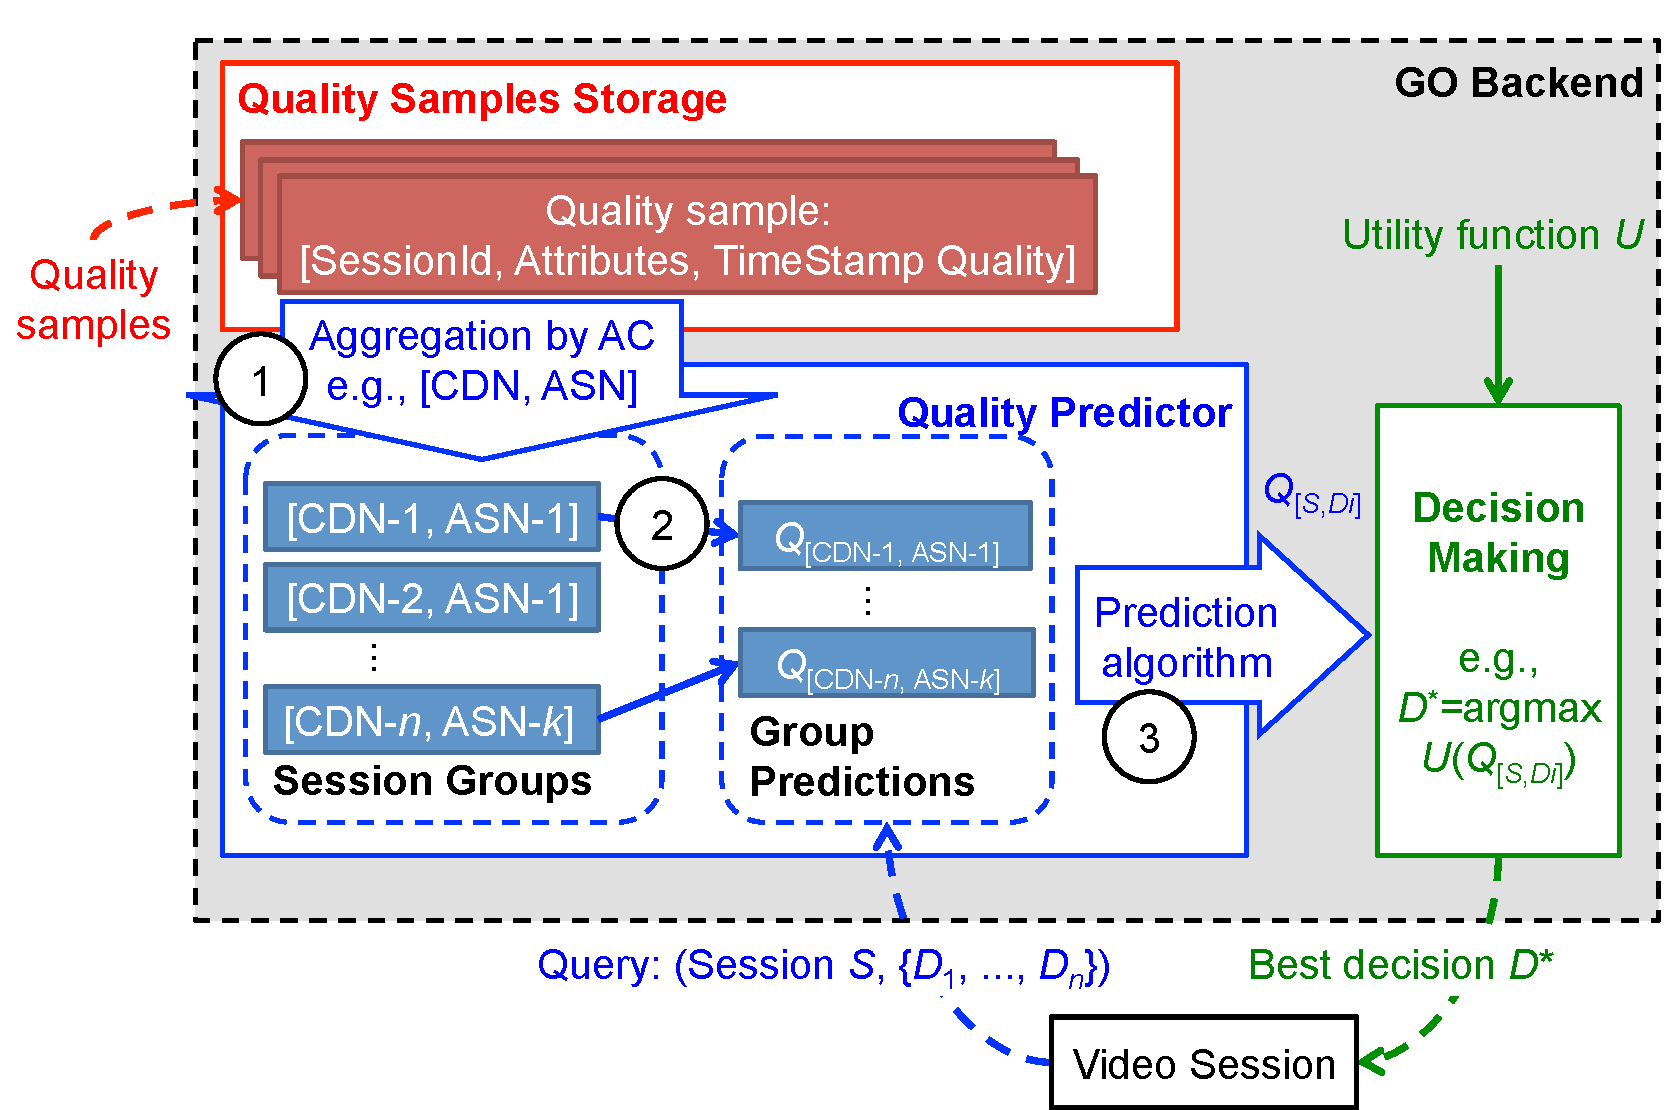
\includegraphics[width=0.3\textwidth] {figures/backend.pdf}
\tightcaption{Schematic overview of GO backend.}
\label{fig:backend}
\end{figure}
}

\tightsubsection{Improving quality with GO}

We first would like to quantify the impact of parameters of scenarios (e.g., performance heterogeneity) on quality improvement with GO.

\begin{figure}[h!]
\centering
\subfigure[CDN performance degradation]
{
        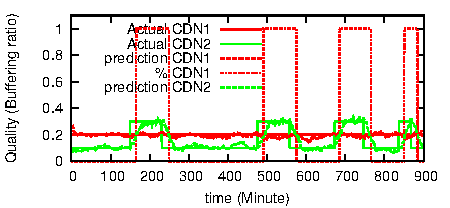
\includegraphics[width=0.4\textwidth]{figures/behavior-evaluation/simple-change.pdf}
	\label{subfig:behavioral:cdn}
}
\subfigure[Impact of bottlenecks]
{
        
\includegraphics[width=0.35\textwidth,height=1.2in]{figures/placeholder.pdf}
	\label{subfig:behavioral:bottleneck}
}
\tightcaption{Behavioral study.}
\label{fig:behavioral}
\end{figure}

\tightsubsubsection{Behavioral study}
\jc{I have a hard time using ``performance'' and ``quality''. Ion, is it correct that we should say CDN performance, quality anywhere else?}
To build confidence in GO and its selection algorithm, we use Type I input (controlled synthetic) to show how decision-making based on prediction behaves in some simple synthetic scenarios where the optimal decisions are clear:

\myparatight{CDN performance degradation} We simulate a scenario in which a sudden change in performance of one group causes GO to switch decision accordingly. Figure~\ref{subfig:behavioral:cdn} shows the behavior of sessions in one ASN when provided with two CDNs to choose from. Assume that buffering ratio is the only considered quality metric. The mean of buffering ratio of CDN1 is stably at 0.2 and that of CDN2 changes between 0.1 and 0.25, with a random interval. Each quality sample of a CDN is generated so that its buffering ratio has a Guassian noise of \fillme deviation from mean. This figure shows clearly that under this configuration, GO is able to switch to the best CDN accordingly with an expected delay (as it uses a 30-minute sliding window). Note that there is always a small amount of randomized traffic, so the change on each decision can be detected. As a side-effect, it takes longer for GO to detect CDN2 from bad quality to good quality than reversely, because the number of samples from CDN2 when it is in bad quality (only randomized traffic) than when it is in good quality (all traffic).

\myparatight{Multiple bottlenecks} We simulate a scenario to compare the effect of CDN performance change on sessions whose quality is bottlenecked by the combination of CDN and ASN.
We create two groups A and B, and two CDNs, CDN1 and CDN2. Sessions of group A belongs to ASN1 and the quality to CDN1 is tably at 0.2 while that to CDN2 changes over time between 0.1 and 0.25 with a random interval. Similarly, sessions of group B belongs to ASN2 and the quality to CDN2 is tably at 0.2 while that to CDN1 changes over time between 0.1 and 0.25 with a random interval. Figure~\ref{subfig:behavioral:cdn} shows the behavior of sessions from each group. The fraction of traffic going to each CDN changes accordingly with the actual CDN performance changes. CDN2 (to ASN1) and CDN1 (to ASN2) change independently and so do the fraction of traffic from each group. This suggests that GO identifies the two groups and optimizing them separately.



\begin{figure*}[t!]
\centering
\subfigure[Buffering ratio]
{
        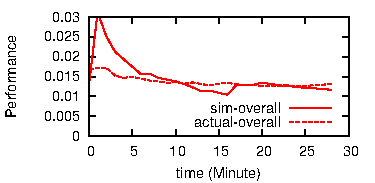
\includegraphics[width=0.23\textwidth]{figures/counterfactual/result-a-overall-metric0.pdf}
}
\subfigure[Average bitrate]
{
        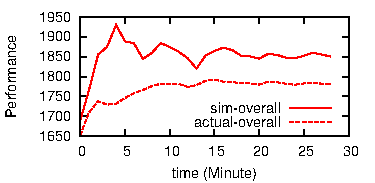
\includegraphics[width=0.23\textwidth]{figures/counterfactual/result-a-overall-metric1.pdf}
}
\subfigure[Join time]
{
        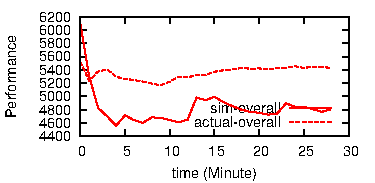
\includegraphics[width=0.23\textwidth]{figures/counterfactual/result-a-overall-metric2.pdf}
}
\subfigure[Start failure rate]
{
        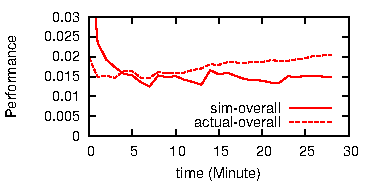
\includegraphics[width=0.23\textwidth]{figures/counterfactual/result-a-overall-metric3.pdf}
}
\tightcaption{\jc{This figure is subject to change! Find a better period.} Counterfactual input. Evaluation under real trace}
\label{fig:counterfactual}
\end{figure*}


\tightsubsubsection{Evaluation under real trace}
We show how GO works in practice in a real trace, in comparison to a naive baseline algorithm that makes random decisions.  To be realistic and get an unbiased evaluation of GO's performance, we use Type II input (couterfactual input); the methodology is described in detail in section \ref{sec:counterfactualtesting}. 

Figure~\ref{fig:counterfactual} shows the performance comparison between GO and random selection over a one day's worth of data. This is from one particular Site whose video can be streamed from three major CDNs in US. Each video is encoded in 6 different levels of bitrates, so that each session has in total 18 candidate decisions to choose from. In this evaluation, GO always select the best decision that gives the highest average bitrate (i.e., targeted quality metric is average bitrate).

Overall, it shows an almost consistent improvement of GO in all metrics, despite that we only consider bitrate. The improvement is \fillme to \fillme for average bitrate, \fillme to \fillme for bitrate, \fillme to \fillme for join time and \fillme to \fillme for start failure rate. Traditinally, people believe that increasing average bitrate is very likely to be at a cost of buffering ratio or join time, as it requires high bandwidth. However, our result suggests that the improvement in average bitrate can be reaches with no cost and even with benefits to other metrics.


\tightsubsubsection{Impact of quality heterogeneity}
To test GO against controlled quality heterogeneity across decisions, we have to identify the true outcome of decisions we did not take, so we use Type III input (randomized trace-driven). Given a session $s$ and one of its decisions $d$, the key challenge is to draw its quality outcome from the distribution ($M_{v_g(s),d}$) that consists of outcomes of the same decision on other sessions that share the same attributes with this session. Remember $v_g(s)$ returns the values on all attributes in $g$ of session $s$, and we use all attributes except for initial bitrate and CDN.
We explore two ways of drawing a the outcome from the distribution. 
\begin{packedenumerate}
	\item {\it Independent method:} The outcome is uniformly at random from $M_{v_g(s),d}$. Its underlying assumption is that we observe all attributes that determine the quality, so that with the same decision, the quality of sessions that match all attribute is random values with unbias noise.
	\item {\it Correlated method:} For a session $s$, if the outcome of $d_1$ is in the $q$-quantile of $M_{v_g(s),d_1}$, the outcome of $d_2$ is also in the $q$-quantile of $M_{v_g(s),d_2}$. Its underlying assumption is that there are unobserved attributes that together determine the quality, so that if the quality from one decision is bad, its quality from another decision will also be relatively bad.
\end{packedenumerate}

Having identified the quality of a session on each decision, we change their quality difference as follows. Let $\Delta$ be the targeted quality heteogeneity. We randomly generated a session $s$ whose its quality on decision $d_1$ is $q_1$ and quality on decision $d_2$ is $q_2$. 
When doing so, we also get the quality prediction when the decision was made. Let $p_1$ be predition of $q_1$ and $p_2$ be prediction of $q_2$. Now, we twist $q_i,p_i$ to be $q_i'.p_i'$, such that (assume $q_1\geq q_2$)
\begin{packeditemize}
	\item (Average bitrate and join time) $q_i'=\delta q_i,p_i'=\delta p_i, i=1,2$ where $\delta=\frac{\Delta}{q_1-q_2}$.
	\item (Buffering ratio and start failure) $p_i'=p_i+\delta_i,q_i'=q_i+\delta_i, i=1,2$ where $\delta_1=\Delta, \delta_2=q_1-q_2$.
\end{packeditemize}
In this way, we not only twist the quality difference to a controlled amount but also preserve the prediction error of original prediction.

Figure~\ref{fig:impact-difference} shows the impact of quality difference $\Delta$ on quality. Since we twist the quality proportionally, it only makes sense to show the relative difference between GO and random selection baseline (i.e., improvement) and between oracle and GO (i.e., room of improvement). The figure shows that \fillme

\begin{figure}[h!]
\centering
 
\includegraphics[width=0.3\textwidth] {figures/placeholder.pdf}
\tightcaption{Impact of quality heterogeneity $\Delta$ (X axis) on quality improvement (Y axis-left) of GO based on random selection, and on room of improvement from GO to oracle (Y axis-right).}
\label{fig:impact-difference}
\end{figure}


%Randomized experimentation in real traces is the most important way to evaluate a decision-making algorithm.  However, real traces have a few limitations.  In real traces, it is impractical to identify an optimal alternative against which to compare GO, so that we can understand how close it is to the best algorithm.  In addition, real traces do not admit simple analysis of the sensitivity of a decision-making algorithm to the changes in scenario parameters.  To remedy these limitations, we generate a synthetic dataset from our real data.  We do this using a simplifying assumption: We fix a set of attributes $g$, and assume that conditional on a session belonging to a group under this AC, its quality outcomes given each decision are statistically independent.  Essentially this amounts to an assumption that we observe all interesting attributes.  \fillme.

%Under this assumption, we can generate a new session from the same distribution that generated a real dataset as follows: Sample uniformly at random from the sessions we observed.  The synthetic session has the same attributes, denoted $a_i$, as the sampled session.  We assign quality outcomes to each possible decision by sampling uniformly at random from the quality outcomes observed for sessions with attributes exactly matching $a_i$.  Crucially, this ensures that quality outcomes in the synthetic scenario are known for any decision, not just the decision that was actually taken for a session.  In particular, it is possible to identify an {\it oracle} for this scenario that makes perfect predictions of quality outcomes for any decision.

% [The following is an unfinished writeup for old synthetic scenario scheme:]
%The scenario is generated as follows: The scenario lasts for $T$ minutes.  Each session is assigned values on four different attributes, $A_0, A_1, B_0,$ and $B_1$, and lasts for $1$ minute.  Each unique attribute combination (i.e. each group) $a$ is associated with some static parameters and some parameters that change over time, which inform the generation of sessions in that group:
%\begin{packedenumerate}
%  \item $n_{a}$: The number of sessions in this group.
%  \item $\mu_{atj}$: The average quality outcome for sessions in this group, when decision $j$ is taken.
%  \item $\sigma_{atj}$: The standard deviation of quality outcomes for sessions in this group, when decision $j$ is taken.
%\end{packedenumerate}
%
%For each minute $t$, sessions are generated as follows: Group $a$ has $n_{a}$ sessions.  The $i$th session in group $a$ has attribute values $a$.  There are $J$ possible decisions; each session has quality outcome $q_{itaj}$ drawn from the distribution $\operatorname{Normal}(\mu_{atj}, \sigma_{atj}^2)$, for each decision $j$.  The actual decision $d_{ita}$ for the session, which is used to populate the quality sample used in GO, is chosen uniformly at random from among the $J$ possible decisions.

%\tightsubsubsection{Evaluation against an oracle using synthetic data}
%Here we compare GO against the oracle (and against a random decision-maker) in our synthetic scenario.  \fillme.
%
%We also check the sensitivity of GO to the true difference in quality between decisions.  We do this by shifting the distribution of true quality outcomes in varying degrees.  \fillme.

\tightsubsection{Impact of prediction accuracy}

Separately from the GO algorithm, it is also interesting to see how prediction error generically impacts quality outcomes. However, it is difficult to model the prediction error. To be representative, we first model the prediction error as an unbiased Gaussian distribution with varying standard deviation. Then, we add random noise to GO's prediction error so as to evaluate impact of GO's degraded prediction accuracy on quality.

\tightsubsubsection{Gaussian prediction error}
  To control the prediction accuracy in real trace, we use randomized trace-driven input. We use the same way to generate sessions and their outcome quality on different decisions, and control the prediction accuracy by generating prediction that deviate from the outcome quality with an independent random Gaussian noise $\epsilon$ (centered at 0) with varying standard deviation $\sigma$: assume $q_i$ is the outcome quality of decision $d_i, i=1,2$
\begin{packeditemize}
	\item (Average bitrate and join time) $p_i=(\epsilon+1)q_i$.
	\item (Buffering ratio and start failure) $p_i=q_i+\epsilon$.
\end{packeditemize}


\begin{figure}[h!]
\centering
 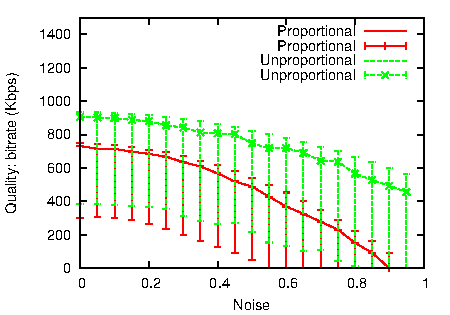
\includegraphics[width=0.3\textwidth] {figures/impact/result-noise-impact.pdf}
\tightcaption{\jc{This figure is subject to change!} Impact of $\sigma$ (X axis) on quality improvement (Y axis-left) of GO based on random selection, and on room of improvement from GO to oracle (Y axis-right). GO prediction gives \fillme Kbps (independent) and \fillme Kbps (correlated), roughly identical to gaussian random noise of standard deviation of \fillme.}
\label{fig:impact-accuracy}
\end{figure}

Figure~\ref{fig:impact-accuracy} quantifies the impact of noise $\epsilon$ on average bitrate. It shows \fillme.

\tightsubsubsection{GO with different prediction error}
Though unbiased Gaussian distribution is a sound way of modeling generic noise, it is not necessary that GO's prediction error follows with Gaussian noise (as shown in Figure~\ref{fig:GO-accuracy-distribution}). 


\begin{figure}[h!]
\centering
 
\includegraphics[width=0.23\textwidth] {figures/placeholder.pdf}
\tightcaption{Prediction error distribution of GO (regarding average bitrate). Not very Gaussian-like.}
\label{fig:GO-accuracy-distribution}
\end{figure}

Instead of using another model, we use Type II (counterfactual) input and add random noise to the prediction made by GO. Again, we use random Guassian noise $\epsilon$ (centered at 0) with varying standard deviation $\epsilon$ to model the added noise: assume $p_i$ is the prediction made by GO for decision $d_i,i=1,2$.
\begin{packeditemize}
	\item (Average bitrate and join time) $p_i'=p_i(1+\epsilon)$.
	\item (Buffering ratio and start failure) $p_i'=p_i+\epsilon, i=1,2$.
\end{packeditemize}

Figure~\ref{fig:impact-accuracy-go} quantifies the impact of noise $\epsilon$ added to GO's prediction on average bitrate.

\begin{figure}[h!]
\centering
 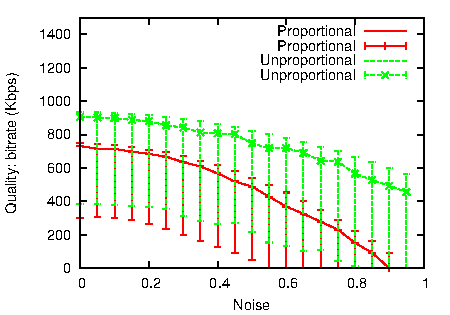
\includegraphics[width=0.3\textwidth] {figures/impact/result-noise-impact.pdf}
\tightcaption{\jc{This figure is subject to change!} Impact of $\sigma$ (X axis) on quality improvement (Y axis-left) of GO based on random selection, and on room of improvement from GO to oracle (Y axis-right). When $\epsilon=0$, the result is identical to GO.}
\label{fig:impact-accuracy-go}
\end{figure}

%Here it is important to identify an oracle predictor as a baseline, so we use the same synthetic scenario as above.  We add random independent Gaussian noise to the oracle's predictions (an admittedly crude model of prediction error) and show how larger amounts of noise impact quality outcomes.  Figure \fillme displays this.  We can see that quality improvement is unaffected by small amounts of prediction inaccuracy but drops off quickly at a (scenario-dependent) threshold \fillme.

%We cannot subtract noise from GO's predictions in a real scenario, since we do not know the true outcome of decisions we did not take.  However, we can {\it add} noise to GO's predictions and observe the impact of {\it worse} prediction on quality outcomes.  As above, we use independent random Gaussian noise of varying magnitude.  Figure \fillme displays this for our synthetic scenario, and figure \fillme displays it for a real trace.  In the synthetic scenario, GO's performance in quality improvement is equivalent to that of an oracle with \fillme random noise.  \henry{We hope to see that decreasing prediction accuracy eventually leads to highly degraded performance.}